% =========================================================
% Required packages in the preamble:
% =========================================================
% \usepackage{booktabs}
% \usepackage{array}
% \usepackage{makecell}
% \usepackage{tabularx}
% \usepackage{float}
% \usepackage{placeins}

% =========================================================
% Appendix
% =========================================================

\clearpage
\onecolumn

\appendix
\section*{Appendix}
\addcontentsline{toc}{section}{Appendix}



\appendix
\section{Exploratory Overview of MSD Features}

\begin{figure}[H]
    \centering
    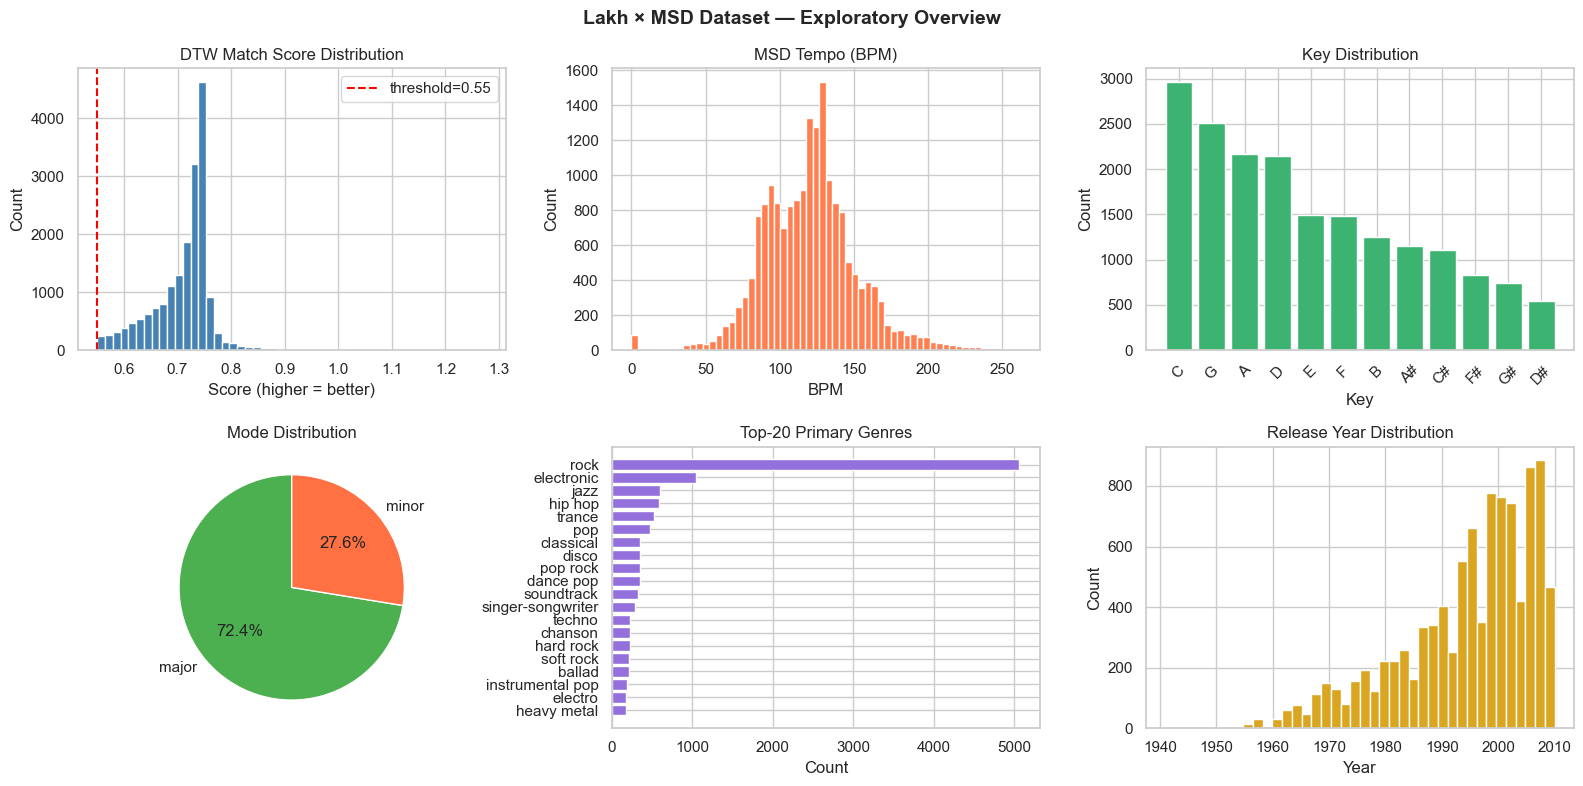
\includegraphics[width=0.99\linewidth]{sec/figures/output1.png}
    \caption{Exploratory Overview of MSD Features.}
    \label{fig:MSD_features}
\end{figure}

% =========================================================
\section{Exploratory Overview of User Taste Profile Filtering Pipeline and Features}


\begin{table}[H]
\centering
\caption{User dataset filtering pipeline statistics.}
\label{tab:data_filtering}
\begin{tabular}{l
                S[table-format=8.0]
                S[table-format=7.0]
                S[table-format=6.0]}
\toprule
\textbf{Step} &
\textbf{Interactions} &
\textbf{Unique Users} &
\textbf{Unique Songs} \\
\midrule
Raw            & 48373586 & 1019318 & 384546 \\
-- Mismatches  & 45795100 & 1019318 & 378309 \\
$\cap$ LMD     & 4243384  & 848243  & 7465   \\
-- Cold-start  & 3048959  & 299156  & 7227   \\
\bottomrule
\end{tabular}
\end{table}

\begin{figure}[H]
    \centering
    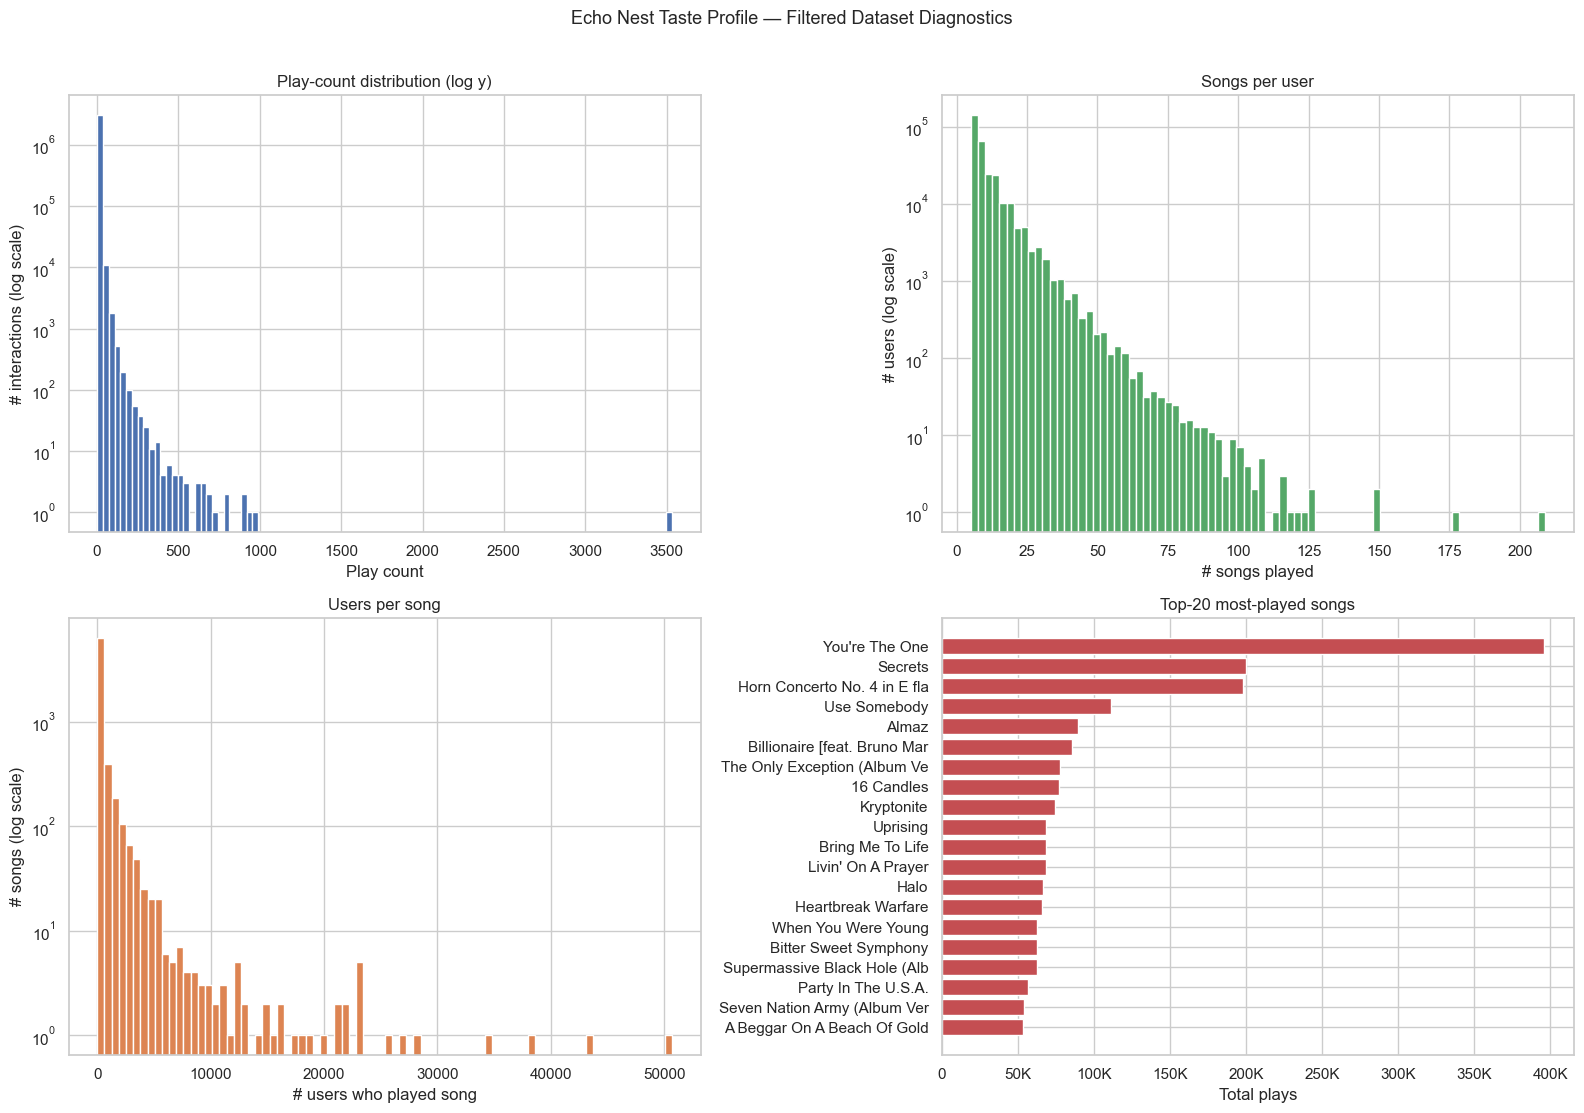
\includegraphics[width=0.99\linewidth]{sec/figures/user_diagnostics.png}
    \caption{Descriptive statistics of the filtered Echo Nest Taste Profile dataset, including the play-count distribution, songs per user, users per song, and the top-20 most-played songs.}
    \label{fig:user_diagnostics}
\end{figure}

% =========================================================
\section{Music-related feature inventory in simple knowledge graph}
% =========================================================
\begin{table*}[t]
\centering
\caption{Music features from MSD and jSymbolic mapping to RDF representation }
\label{tab:kg_features}
\scriptsize
\setlength{\tabcolsep}{3pt}
\renewcommand{\arraystretch}{1.15}

\begin{tabular}{
>{\bfseries\ttfamily\raggedright\arraybackslash}p{3.2cm}
>{\raggedright\arraybackslash}p{4.6cm}
>{\raggedright\arraybackslash}p{1.2cm}
>{\raggedright\arraybackslash}p{3.8cm}
>{\raggedright\arraybackslash}p{3.3cm}
}
\hline
\textbf{Feature Name} & \textbf{Description} & \textbf{Origin} & \textbf{RDF Term} & \textbf{Storage Type} \\
\hline

track\_id & Unique MSD track identifier used as the primary URI for the track node & MSD & mo:uuid (literal on track node) & Literal (xsd:string) \\
song\_id & Echo Nest song identifier used for cross-referencing with taste profile & MSD & dct:identifier (literal on track node) & Literal (xsd:string) \\
artist\_id & MSD canonical artist identifier used as the artist node URI & MSD & URI slug (artist: namespace) & Named Node (mo:Performer) \\
artist\_mbid & MusicBrainz cross-reference identifier for the artist & MSD & mo:musicbrainz\_guid & Literal (xsd:string) \\
artist\_name & Display name of the artist & MSD & foaf:name & Literal (xsd:string) \\
title & Title of the track & MSD & dct:title & Literal (xsd:string) \\
album\_name & Name of the release/album the track belongs to & MSD & dct:isPartOf & Literal (xsd:string) \\
year & Release year of the track & MSD & dct:date & Literal (xsd:gYear) \\
key & Musical key of the track (C C\# D ... B) & MSD & mrc:hasKey & Named Node (mrc:Key individual) \\
key\_confidence & Confidence score of the key detection (0--1) & MSD & mrc:keyConfidence & Literal (xsd:double) \\
mode & Modality of the track (Major or Minor) & MSD & mrc:hasMode & Named Node (mrc:Mode individual) \\
mode\_confidence & Confidence score of the mode detection (0--1) & MSD & mrc:modeConfidence & Literal (xsd:double) \\
loudness & Overall loudness of the track in decibels & MSD & mrc:loudness & Literal (xsd:double) \\
duration & Duration of the track in seconds & MSD & mo:duration & Literal (xsd:double) \\
primary\_genre & Primary genre tag of the artist (weight = 1.0) & MSD & mrc:hasGenre (via artist) & Named Node (mrc:Genre individual) \\
top3\_genres & Top 3 genre tags of the artist with rank-based weights & MSD & mrc:hasGenre (via artist) & Named Node (mrc:Genre individual) \\
artist\_terms & Full list of MSD genre/style tags with published weights & MSD & mrc:hasGenre (via artist) & Named Node (mrc:Genre individual) \\
midi\_instrument\_names & List of General MIDI instrument names present in the MIDI file & MIDI (LMD) & mo:instrument (via performance) & Named Node (mo:Instrument individual) \\
tempo (Mean\_Tempo / msd\_tempo) & Mean BPM of the track; used to derive the categorical tempo class & jSymbolic / MSD & mo:tempo & Literal (xsd:double) \\
Tempo class & Categorical tempo marking derived from BPM (e.g. Allegro Andante) & Derived & mrc:hasTempoClass & Named Node (mrc:TempoClass individual) \\
Mean\_Tempo & Mean tempo computed by jSymbolic & jSymbolic & mrc:meanTempo & Literal (xsd:double) \\
Initial\_Tempo & Tempo at the start of the piece & jSymbolic & mrc:initialTempo & Literal (xsd:double) \\
Tempo\_Variability & Variability of tempo across the piece & jSymbolic & mrc:tempoVariability & Literal (xsd:double) \\
Note\_Density & Average number of notes per second & jSymbolic & mrc:noteDensity & Literal (xsd:double) \\
Average\_Note\_Duration & Mean duration of individual notes & jSymbolic & mrc:averageNoteDuration & Literal (xsd:double) \\
Amount\_of\_Staccato & Proportion of notes that are staccato & jSymbolic & mrc:amountOfStaccato & Literal (xsd:double) \\
Amount\_of\_Arpeggiation & Degree of arpeggiated melodic motion & jSymbolic & mrc:amountOfArpeggiation & Literal (xsd:double) \\
Chromatic\_Motion & Proportion of melodic intervals that are semitones & jSymbolic & mrc:chromaticMotion & Literal (xsd:double) \\
Chord\_Duration & Mean duration of chords & jSymbolic & mrc:chordDuration & Literal (xsd:double) \\
Average\_Number\_of\_Independent\_Voices & Mean number of simultaneous melodic voices & jSymbolic & mrc:averageNumberOfIndependentVoices & Literal (xsd:double) \\
Average\_Note\_to\_Note\_Change\_in\_Dynamics & Mean change in dynamics between consecutive notes & jSymbolic & mrc:averageNoteToNoteChangeInDynamics & Literal (xsd:double) \\

\hline
\end{tabular}
\end{table*}